\documentclass{article}

% Language setting
% Replace `english' with e.g. `spanish' to change the document language
\usepackage[english]{babel}

% Set page size and margins
% Replace `letterpaper' with `a4paper' for UK/EU standard size
\usepackage[letterpaper,top=2cm,bottom=2cm,left=3cm,right=3cm,marginparwidth=1.75cm]{geometry}

% Useful packages
\usepackage{amsmath}
\usepackage{float}
\usepackage{graphicx}
\usepackage[colorlinks=true, allcolors=blue]{hyperref}

\title{Računalniška grafika zapiski}
\author{Tim Hajdinjak}

\begin{document}
\maketitle

\section{Matematične osnove}

Osnovni pojmi, brez katerih žal ne gre

\begin{itemize}
\item stolpčna matrika: $\begin{bmatrix} 2,9 \\ -4,6 \\ 0 \end{bmatrix}$
\item vrstična matrika:  $\begin{bmatrix} 12,5 & -9,32 & 0 \end{bmatrix}$
\item transponiranje: pomeni zamenjavo osi dveh matrik: $\begin{bmatrix} 1,3 & -4,1 & 0,0 \end{bmatrix}^T = \begin{bmatrix} 1,3 \\ -4,1 \\ 0,0 \end{bmatrix}$
\item enakost matrik: dve matriki sta si enaki, če imata enako število elementov po obeh oseh, in so vsi vsebovani elementi na enakih mestih
\item vektor: predstavljen kot matrika, pomeni premik iz točke v točko, nimajo lokacije, smer gibanja
\item seštevanje matrik: $a + b = c \iff c_i = a_i + b_i$, intuitivno: 
\begin{figure}[H]
\centering
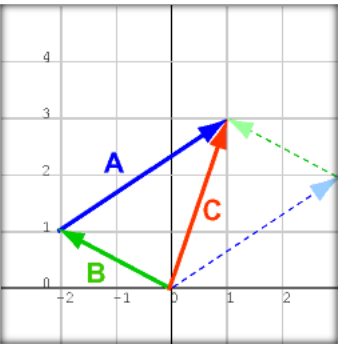
\includegraphics[width=25mm]{src/sestevanje_vektorjev.png}
\caption{Geometrijsko sestevanje vektorjev. (iz repa vektorja 1 na glavo vektorja 2)}
\end{figure}
\item enota za seštevanje: $a + 0 = 0 + a = a \iff \begin{bmatrix} 3 & -1 \end{bmatrix} + \begin{bmatrix} 0 & 0 \end{bmatrix} = \begin{bmatrix} 3 & -1 \end{bmatrix}$
\item odštevanje matrik: $a - b = c \iff c_i = a_i - b_i$
\item množenje s skalarjem: $\alpha * a = b \iff b_i = \alpha * a_i$
\item inverz za seštevanje: $a - a = a + -a = a + (-1)a=0 \iff \begin{bmatrix} 2 & 5 \end{bmatrix} - \begin{bmatrix} 2 & 5 \end{bmatrix} = \begin{bmatrix} 2 & 5 \end{bmatrix} + \begin{bmatrix} -2 & -5 \end{bmatrix}=\begin{bmatrix} 0 & 0 \end{bmatrix}$
\item NORMA oz. dolžina vektorja: $h = \begin{bmatrix} x \\ y \end{bmatrix} \Longrightarrow \lVert h \rVert = \sqrt{x^2 + y^2}, oz. \lVert a \rVert = \sqrt{\sum_{i=1}^n a_i^2}$ (L2 norm oz. evklidska razdalja). Splošna norma: $\lVert a \rVert_p = \sqrt[p]{\sum_{i=1}^n |a_i|^p}$. Torej, če na izpitu reče druga splošna norma, namesto p pišeš 2. Neskončna norma $\to$ dolžina se bliža maksimalni vrednosti vektorja. 
\item enotski vektor, pomeni vektor dolžine 1, $\lVert e \rVert = 1$
\item normalizacija: $v = \begin{bmatrix} v_x \\ v_y \\ v_z \end{bmatrix} \Longrightarrow \hat{v} = v / \lVert v \rVert = \begin{bmatrix} v_x/\lVert v \rVert \\ v_y/\lVert v \rVert \\ v_z/\lVert v \rVert \end{bmatrix}, \hat{v} = $ enotskost vektorja (podajo samo smer), posamezne elemente vektorja delimo z njegovo dolžino.
\item skalarni produkt: $u = \begin{bmatrix} u_0 \\ u_1 \\ u_2 \end{bmatrix}, v = \begin{bmatrix} v_0 \\ v_1 \\ v_2 \end{bmatrix} \Longrightarrow u * v = u_0*v_0 + u_1*v_1 + u_2*v_2$. Pravimo mu tudi "detektor pravokotnosti", saj:
\begin{enumerate}
    \item $u*v = 0 \to$ vektorja pravokotna
    \item $u*v < 0 \to$ iztegnjen kot
    \item $u*v > 0 \to$ ostri kot
    \item $\hat{a} * \hat{b} \to$ vrednosti med $[-1, 1],-1 = 180^\circ, 0 = 90^\circ, 1 = 0^\circ$
\begin{figure}[H]
\centering
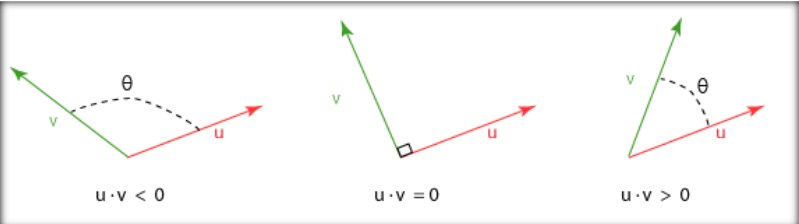
\includegraphics[width=100mm]{src/ortogonalnost.png}
\caption{2 vektorja sta ortogonalna, če je skalarni produkt enak 0 (oz. sta si pravokotna)}
\end{figure}
\begin{figure}[H]
\centering
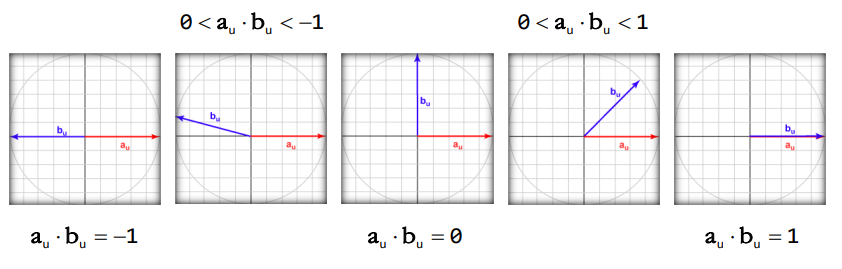
\includegraphics[width=100mm]{src/skalarni_produkt_enotskih_vektorjev.png}
\caption{Skalarni produkt enotskih vektorjev}
\end{figure}
\end{enumerate}
Še par pravil oz. posebnosti pri skalarnih produktih:
\begin{itemize}
    \item $u * v = \lVert u \rVert * \lVert v \rVert * \cos{\alpha}$
    \item $v * v = \lVert v  \rVert^2$, norma
    \item $u * 0 = 0 * u = 0$, skalarni produkt z vektorjem 0
    \item $0 * 0 = 0$, skalarni produkt vektorja 0
    \item $u * v = v * u$, komutativnost
    \item $u * (v+w) = u*v + u*w$, distributivnost za seštevanje
    \item $(\alpha u)*v = u * (\alpha v) = \alpha * (u * v)$, homogenost za množenje s skalarjem
    \item $u \perp v \iff u * v = 0$, skalarni produkt ortogonalnih (pravokotnih) vektorjev
    \item Asociativnost: nedefinirana operacija, vrstni red je pomemben
\end{itemize}
\item linearna neodvisnost, projekcija vektorja na vektor: $kv = \lVert w \rVert (w_u * v_u)*v_u$
\begin{figure}[H]
\centering
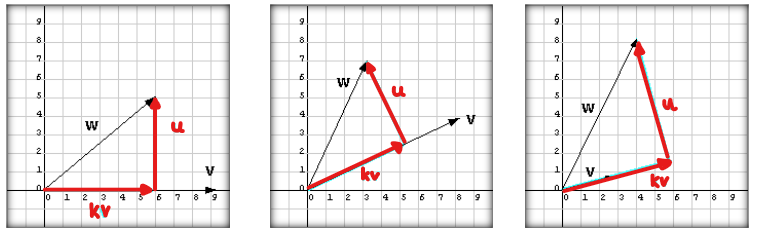
\includegraphics[width=100mm]{src/projekcija_vektorja_na_vektor.png}
\caption{Projekcija vektorja na vektor}
\end{figure}
Postopek pri linearne neodvisnost:
\begin{enumerate}
    \item Izračunaj dolžine vektorjev: $\lVert w \rVert = w * w, \lVert v \rVert = v * v$ 
    \item Izračunaj enotske vektorje: $w_u = w/ \lVert w \rVert, v_u = v/ \lVert v \rVert$
    \item Izračunaj kosinus kota med vektorji: $\cos{\alpha} = w_u * v_u$
    \item Združi v projekcijo: $kv = \lVert w \rVert (w_u * v_u)*v_u$
    \item Izračunaj ortogonalni vektor: $u = w - kv$
\end{enumerate}
\item Vektorski produkt: $u = \begin{bmatrix} u_x \\ u_y \\ u_z \end{bmatrix}, v = \begin{bmatrix} v_x \\ v_y \\ v_z \end{bmatrix}, u \times v = \begin{bmatrix} u_yv_z - u_zv_y \\ u_zv_x - u_xv_z \\ u_xv_y - u_yv_x \end{bmatrix}$
\begin{figure}[H]
\centering
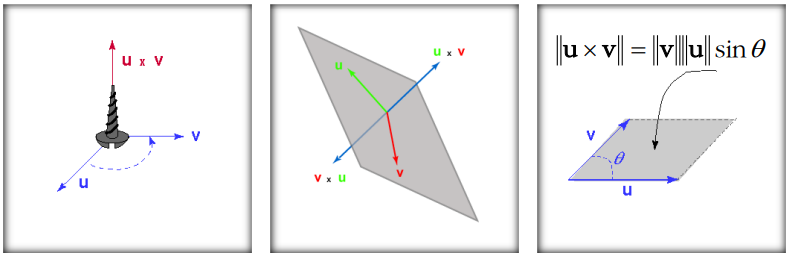
\includegraphics[width=100mm]{src/vektorski_produkt.png}
\caption{Vektorski produkt intuitivno}
\end{figure}
\begin{figure}[H]
\centering
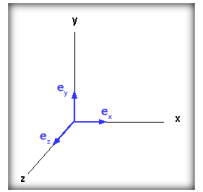
\includegraphics[width=30mm]{src/enotski_vektorji.png}
\caption{Enotski vektorji, ki tvorijo prostor $R^3$, imajo normo (dolžino) 1 in so vzajemno pravokotni. Pri tem je $e_x = (1,0,0), e_y = (0,1,0), e_z = (0,0,1)$}
\end{figure}
Zakonitosti pri vektorskem produktu:
\begin{enumerate}
    \item $u \times v = -(v \times u)$, antikomutativnost
    \item $u \times (v + w) = u \times v + u \times w$, distributivnost za seštevanje
    \item $(\alpha u) \times v = u \times (\alpha v) = \alpha(u \times v)$, homogenost za množenje s skalarjem
    \item Asociativnost ne obstaja:  $u \times (v \times w) \not = (u \times v) \times w$
    \item $u \parallel v \iff u \times v = 0$, vektorski produkt kolinearnih vektorjev
    \item $u \times 0 = 0 \times v = 0$, vektorski produkt vektorja 0
    \item $0 \times 0 = 0$, vektorski produkt z vektorjem 0
    \item $e_x \times e_y = e_z, e_y \times e_z = e_x, e_z \times e_x = e_y$, vektorski produkt koordinatnih osi, zanimivost: vidimo lahko desno pravilo
\end{enumerate}
\item Splošna matrika, notacija: $A_{m \times n} = \begin{bmatrix}
    a_{11} & a_{12} & \cdots & a_{1n} \\
    a_{21} & a_{22} & \cdots & a_{2n} \\
    \vdots & \vdots & \ddots & \vdots \\
    a_{m1} & a_{m2} & \cdots & a_{mn}
\end{bmatrix}$
\item Seštevanje matrik: $A + B = C \iff c_{ij} = a_{ij} + b_{ij}$, primer: $\begin{bmatrix} 2 & 0 \\ -1 & 2 \\ 3 & 5 \end{bmatrix} + \begin{bmatrix} 
 1 & 3 \\ -1 & 2 \\2 & -1 \end{bmatrix} = \begin{bmatrix} 3 & 3 \\ -2 & 4 \\ 5 & 4 \end{bmatrix}$
 Zakonitosti pri seštevanju splošnih matrik:
 \begin{enumerate}
     \item Možno le, če sta matriki enakih dimenzij! 
     \item $A + B = B + A$, komutativnost
     \item $(A + B) + C = A + (B + C)$, asociativnost
     \item $A + 0 = 0 + A = A$, enota za seštevanje
     \item $A - A = A + (-1)A = 0$, inverz za seštevanje
 \end{enumerate}
\item Množenje matrik s skalarjem: $\alpha A = B \iff b_{ij} = \alpha a_{ij}$, primer: $3 * \begin{bmatrix} 2 & 0 \\ -1 & 2 \\ 3 & 5 \end{bmatrix} = \begin{bmatrix} 6 & 0 \\ -3 & 6 \\ 9 & 15 \end{bmatrix}$
Zakonitosti pri množenju matrik s skalarjem:
\begin{enumerate}
    \item $\alpha (A + B) = \alpha A + \alpha B$, distributivnost seštevanja matrik
    \item $(\alpha + \beta)A = \alpha A + \beta A$, distributivnost seštevanja skalarjev
    \item $(\alpha \beta)A = \alpha (\beta A)$, asociativnost
    \item $(-1)A = -A$, množenje s skalarjem -1
\end{enumerate}
\item Množenje matrik: $A_{n \times m}B_{m \times p} = C_{n \times p} \iff c_{ij} = \sum_{k=1}^m a_{ik}b_{kj}$
\begin{figure}[H]
\centering
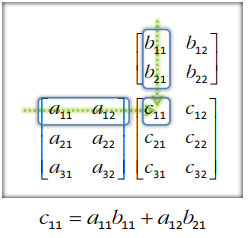
\includegraphics[width=40mm]{src/mnozenje_matrik.png}
\caption{Miselni vzorec za množenje splošnih matrik}
\end{figure}
Zakonitosti pri množenju matrik:
\begin{enumerate}
    \item $AB \not = BA$, komutativnost ne velja
    \item $(AB)C = A(BC)$, asociativnost
    \item $A(B + C) = AB + AC$, distributivnost za seštevanje
    \item $(A + B)C = AC + BC$, distributivnost za seštevanje
    \item $(\alpha A)B = A(\alpha B) = \alpha (AB)$, homogenost za množenje s skalarjem
    \item $0A = 0$, množenje s skalarjem 0
    \item $A0 = 0A = 0$, množenje z matriko 0
\end{enumerate}
\item Enota za množenje oz. identiteta: $I_n = \begin{bmatrix} 
1 & 0 & 0 & \cdots & 0 \\ 0 & 1 & 0 & \cdots & 0 \\ 0 & 0 & 1 & \cdots & 0 \\ \vdots & \vdots & \vdots & \ddots & \vdots \\ 0 & 0 & 0 & \cdots & 1 \end{bmatrix}_{n \times n}$, 1 po diagonali
\begin{enumerate}
    \item $AB = BA = I \iff B = A^{-1}$
    \item $(ABC)^{-1} = C^{-1}B^{-1}A^{-1}$, inverz za množenje
\end{enumerate}
\item Transponiranje: $A^T = B \iff b_{ij} = a_{ji}$
Lastnosti transponiranja:
\begin{enumerate} 
    \item $(A^T)^T = A$
    \item $(\alpha A)^T = \alpha A^T$
    \item $(A + B)^T = A^T + B^T$
    \item $(ABC)^T = C^TB^TA^T$
    \item $(A^{-1})^T = (A^T)^{-1}$
\end{enumerate}
\end{itemize}

\section{Transformacije in homogene koordinate}

\begin{itemize}
    \item Teselacija je matematični koncept, ki se nanaša na prekrivanje ravnine z enakimi (homogenimi, urejeno) ali različnimi (nehomogenimi, neurejeno) geometrijskimi oblikami brez prekrivanja. Te oblike so lahko trikotniki, kvadrati, šestkotniki,..., ki se ponavljajo na urejen način, da zapolnijo celotno površino. Več oblik dodajamo, bolj natančen bo naš objekt. 
    \item Mozaičenje: razbitje površine na manjše koščke.
    \item LOD (Level of Detail), tehnika, kjer se uporabljajo različne različice 3D modela z različnimi stopnjami podrobnosti glede na razdaljo modela od kamere. Torej, ko je objekt blizu kamere, se uporablja višji nivo (več teselacije), ko pa je daleč, pa nižji (manj teselacije). Namen LOD je izboljšati učinkovitost izrisa ter optimizacijo delovanja sistema. 
    \item Ko pa aplikacija oz. program določi natančnost objektov, jih game engine uredi tako, da zmanjša število podatkov (manj teselacije).
    \item Vedno delamo z ogljišči, vse ostalo je potem posledica. S trikotniki opišemo ploskovne površine. 
    \item Linearna transformacija: $p' = f(p)$, preslikave, ki preslikajo eno točko v drugo.
    \item Razteg/skaliranje: enakomeren (uniformen) oz. neenakomeren (neuniformen)
    \begin{figure}[H]
    \centering
    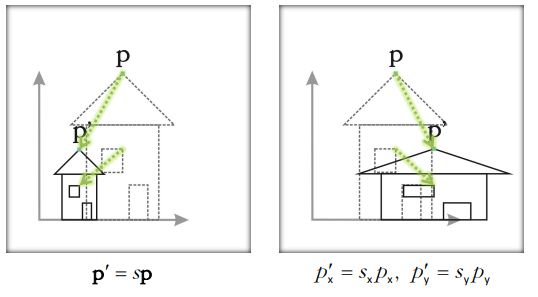
\includegraphics[width=100mm]{src/razteg_skaliranje.png}
    \caption{Primer enakomernega ter neenakomernega skaliranja}
    \end{figure}
    \item Striženje: spreminjamo eno izmed osi  na podlagi vrednosti druge osi. Če želimo striženje za kot $\phi$, uporabimo kotangens kota.
    \begin{figure}[H]
    \centering
    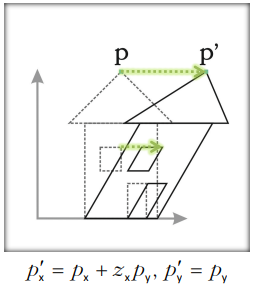
\includegraphics[width=40mm]{src/strizenje.png}
    \caption{Primer striženja}
    \end{figure} 
    \item Zrcaljenje: zrcaljenje čez koordinatne osi. Če zrcalimo dvakrat, dobimo isto. Če želimo zrcalit čez os $x = y$, uporabimo: $p_x' = p_y$ in $p_y' = p_x$ (x in y os se zamenjata). "Razteg z negativnim številom"
    \begin{figure}[H]
    \centering
    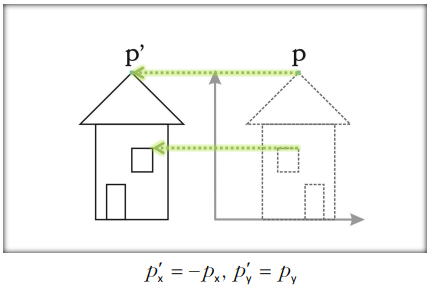
\includegraphics[width=75mm]{src/zrcaljenje.png}
    \caption{Primer zrcaljenja preko Y osi}
    \end{figure} 
    \item Vrtenje: vedno vrtimo v nasprotno smer urinega kazalca okrog izhodišča. 
    \begin{figure}[H]
    \centering
    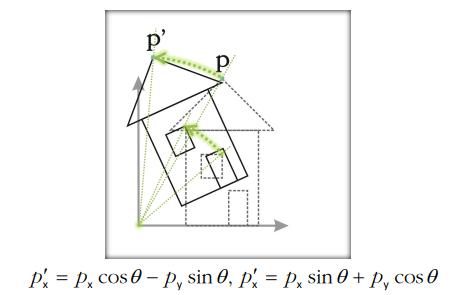
\includegraphics[width=75mm]{src/vrtenje.png}
    \caption{Primer vrtenja okrog izhodišča}
    \end{figure}     
    Izpeljava:
    \begin{enumerate}
        \item Zapis s polarnimi koordinatami: \\
        $p_x = \lVert p \rVert \cos{\phi}$ \\
        $p_y = \lVert p \rVert \sin{\phi}$
        \item Vrtenje v polarnih koordinatah: (povemo kot in radij (oddaljenost od izhodišča)) \\
        $p_x' = \lVert p \rVert \cos{(\phi + \theta)}$ \\
        $p_y' = \lVert p \rVert \sin{(\phi + \theta)}$
        \item Adicijski izreki kotnih funkcij: ($\cos{(\phi + \theta)} = \cos{\phi}\cos{\theta}$, enako za $sin$) \\
        $p_x' = \lVert p \rVert \cos{\phi} \cos{\theta} - \lVert p \rVert \sin{\phi} \sin{\theta}$ \\
        $p_y' = \lVert p \rVert \cos{\phi} \sin{\theta} + \lVert p \rVert \sin{\phi} \cos{\theta}$
        \item Pretvorba v kartezične koordinate: (iz 1. izrazimo $\lVert p \rVert$, in se 3. pokrajša:)\\
        $p_x' = p_x \cos{\theta} - p_y \sin{\theta}$ \\
        $p_y' = p_x \sin{\theta} + p_y \cos{\theta}$
    \end{enumerate}
    \item Linearne transformacije, omenjene zgoraj, lahko zapišemo kot matrike:
    \begin{itemize}
        \item Nova točka = matrika $*$ točka
        \item Matrika 2x2 za 2D
        \item Matrika 3x3 za 3D
    \end{itemize}
    \begin{enumerate}
        \item $p' = Mp$, nova točka = matrika $*$ točka
        \item $S(s_x, s_y) = \begin{bmatrix} s_x & 0 \\ 0 & s_y \end{bmatrix}$, za skaliranje gremo vzdolž padajoče diagonale
        \item $Z(z_x, z_y) = \begin{bmatrix} 1 & z_x \\ z_y & 1 \end{bmatrix}$, striženje za nek faktor
        \item $Z(\theta, \phi) = \begin{bmatrix} 1 & \cot{\theta} \\ \cot{\phi} & 1 \end{bmatrix}$, striženje za kot $\phi$  
        \item $M_x = \begin{bmatrix} -1 & 0 \\ 0 & 1 \end{bmatrix}$, zrcaljenje čez Y os
        \item $M_y = \begin{bmatrix} 1 & 0 \\ 0 & -1 \end{bmatrix}$, zrcaljenje čez X os
        \item $M_{x=y} = \begin{bmatrix} 0 & 1 \\ 1 & 0 \end{bmatrix}$, zrcaljenje čez os x=y    
        \item $R(\theta) = \begin{bmatrix} \cos{\theta} & -\sin{\theta} \\ \sin{\theta} & \cos{\theta} \end{bmatrix}$, rotiranje za kot $\theta$ v 2D prostoru, za obe koordinati X in Y
        \item Vrtenje v 3D prostoru: $p' = R_{x|y|z}(\theta)p$. Tukaj v bistvu vrtimo objekt preko neke koordinatne osi A, da se giblje v ravnini koordinatnih osi B in C. Primer: če vrtimo okoli koordinatne osi Z, se bo objekt vrtel preko X in Y koordinate, Y = X in Z ter X = Y in Z. To pomeni, da če vrtimo preko, ne vem, koordinatne osi Z, bomo v 3x3 matriki (ker smo v 3D), dali zadnjo vrstico in stolpec (oz. vrstici in stolpcu, ki pripada tej koordinatni osi), vse 0, razen en element na 1, kjer se stikata. \\ Primer: $R_z(\theta) = \begin{bmatrix} 
 \cos{\theta} & -\sin{\theta} & 0 \\ \sin{\theta} & \cos{\theta} & 0 \\ 0 & 0 & 1 \end{bmatrix}$ (matrika, ki zavrti objekt preko koordinatne osi Z), in preko zgornje enačbe dobimo: $p' = R_{z}(\theta)p = \begin{bmatrix} p_x \cos{\theta} - p_y \sin{\theta} \\ p_x \sin{\theta} + p_y \cos{\theta} \\ p_z \end{bmatrix}$. Matriki za preostali koordinatni osi X in Y: $R_x(\theta) = \begin{bmatrix} 1 & 0 & 0 \\ 0 & \cos{\theta} & -\sin{\theta} \\ 0 & \sin{\theta} & \cos{\theta} \end{bmatrix}$, $R_y(\theta) = \begin{bmatrix} 
\cos{\theta} & 0 & \sin{\theta} \\ 0 & 1 & 0 \\ -\sin{\theta} & 0 &\cos{\theta} \end{bmatrix}$
    \end{enumerate}
\end{itemize}

\subsection{Afine transformacije}
\begin{itemize}
    \item $p' = Mp + t$, linearne transformacije s premiki
    \item $v = \begin{bmatrix} v_x \\ v_y \\ v_z \end{bmatrix} = v_xe_x + v_ye_y + v_ze_z$, vektor zapisan tudi s pomočjo enotskih vektorjev
    \item $p = \begin{bmatrix} p_x \\ p_y \\ p_z \\ 1 \end{bmatrix} = p_xe_x + p_ye_y + p_ze_z + o$, dodatek homogene koordinate (1 = točka, 0 = vektor), z njimi lahko izvajam premike (točka je 1, ker je odvisna od izhodišča (zato to prištejemo), vektor pa samo navaja premike (ni vezan na izhodišče sistema))
    \item $p_h = \begin{bmatrix} wp_x \\ wp_y \\ wp_z \\ w \end{bmatrix} = wp_xe_x + wp_ye_y + wp_ze_z + wo$, če pa želimo prehod iz homogene v nehomogene elemente: vsako koordinato delimo z $w$
    \item $p_h = \begin{bmatrix} p_x \\ p_y \\ p_z \\ 1 \end{bmatrix}$, $v_h = \begin{bmatrix} v_x \\ v_y \\ v_z \\ 0 \end{bmatrix}$, $p_h' = p_h + v_h = \begin{bmatrix} p_x + v_x \\ p_y + v_y \\ p_z + v_z \\ 1 \end{bmatrix}$, dobim točko, če pa odštejem, dobim vektor ("točki lahko prištejemo vektor in dobimo točko")
    \item Premik v homogenih koordinatah: $p' = T(t)p$, T = translate, premaknemo točko za točko $t$. Primer: $p = \begin{bmatrix} 
p_x \\ p_y \\ p_z \\ 1 \end{bmatrix}, t = \begin{bmatrix} 
t_x \\ t_y \\ t_z \\ 0 \end{bmatrix} \Longrightarrow p' = \begin{bmatrix} 
p_x' \\ p_y' \\ p_z' \\ 1 \end{bmatrix} = \begin{bmatrix} 
1 & 0 & 0 & t_x \\ 0 & 1 & 0 & t_y \\ 0 & 0 & 1 & t_z \\ 0 & 0 & 0 & 1 \end{bmatrix} \begin{bmatrix} p_x \\ p_y \\ p_z \\ 1 \end{bmatrix} = \begin{bmatrix} p_x + t_x \\ p_y + t_y \\ p_z + t_z \\ 1 \end{bmatrix}$ \\ Za premike obstaja inverzna operacija, s tem vrnemo neko točko nazaj kjer je bila: \\ $T(t) = \begin{bmatrix} 
1 & 0 & 0 & t_x \\ 0 & 1 & 0 & t_y \\ 0 & 0 & 1 & t_z \\ 0 & 0 & 0 & 1 \end{bmatrix}$, inverz: $T(t)^{-1} = \begin{bmatrix} 
1 & 0 & 0 & -t_x \\ 0 & 1 & 0 & -t_y \\ 0 & 0 & 1 & -t_z \\ 0 & 0 & 0 & 1 \end{bmatrix}$
    \item Razteg v homogenih koordinatah: $p' = S(s_x, s_y, s_z)p$, S = scale: \\ $p = \begin{bmatrix} 
p_x \\ p_y \\ p_z \\ 1 \end{bmatrix} \Longrightarrow p' = \begin{bmatrix} 
p_x' \\ p_y' \\ p_z' \\ 1 \end{bmatrix} = \begin{bmatrix} 
s_x & 0 & 0 & 0 \\ 0 & s_y & 0 & 0 \\ 0 & 0 & s_z & 0 \\ 0 & 0 & 0 & 1 \end{bmatrix} \begin{bmatrix} p_x \\ p_y \\ p_z \\ 1 \end{bmatrix} = \begin{bmatrix} s_xp_x \\ s_yp_y \\ s_zp_z \\ 1 \end{bmatrix}$ \\ Raztegi poznajo tudi inverzno operacijo: $S(s_x, s_y, s_z)^{-1} = S(\frac{1}{s_x},\frac{1}{s_y}, \frac{1}{s_z})$
    \item Vrtenje v homogenih koordinatah (3D): $p' = R(\theta)p$, R = rotate, rotiramo za kot $\theta$, na določeni koord. osi: \\
    $R_x(\theta) = \begin{bmatrix} 1 & 0 & 0 & 0 \\ 0 & \cos{\theta} & -\sin{\theta} & 0 \\ 0 & \sin{\theta} & \cos{\theta}  & 0 \\ 0 & 0 & 0 & 1\end{bmatrix}$, $R_y(\theta) = \begin{bmatrix} 
\cos{\theta} & 0 & \sin{\theta} & 0 \\ 0 & 1 & 0 & 0\\ -\sin{\theta} & 0 &\cos{\theta} & 0 \\ 0 & 0 & 0 & 1 \end{bmatrix}$, $R_z(\theta) = \begin{bmatrix} \cos{\theta} & -\sin{\theta} & 0 & 0 \\ \sin{\theta} & \cos{\theta} & 0 & 0\\ 0 & 0 & 1 & 0 \\ 0 & 0 & 0 & 1\end{bmatrix}$ \\ 
Vrtenje ima tudi inverzno operacijo, vendar samo, če poznamo kot: $R(\theta)^{-1} = R(-\theta) = R(\theta)^T$
    \item Striženje v homogenih koordinatah: $p' = Z(z_1,\dots,z_6)p$, Z = shear, $Z(z_1,\dots,z_6) = \begin{bmatrix} 1 & z_1 & z_2 & 0 \\ z_3 & 1 & z_4 & 0 \\ z_5 & z_6 & 1 & 0 \\ 0 & 0 & 0 & 1 \end{bmatrix}$ \\ V 2D prostoru gre striženje po določeni koordinatni osi, v 3D pa po vzdolž ravnine.
    \item Ortonorminirana baza: vektorji so med seboj pravokotni: če so matrike ortonorminirane, lahko za izračun inverza samo transponiramo
    \item Transformacijska matrika: matrika, v kateri lahko hkrati delamo več operacij
    \begin{figure}[H]
    \centering
    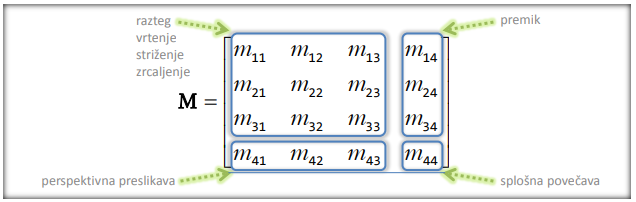
\includegraphics[width=100mm]{src/transformacijska_matrika.png}
    \caption{Definicija transformacijske matrike}
    \end{figure}   
\end{itemize}

\subsection{Veriženje transformacij}
\begin{itemize}
    \item $p' = M_3M_2M_1p$, najprej $M_1$, nato $M_2$ ter šele nato $M_3$ (najprej tista, ki je najbližja točki)
    \item Eulerjevi koti: $R_E(\theta_h, \theta_p, \theta_r) = R_z(\theta_r)R_x(\theta_p)R_y(\theta_h)$
    \begin{figure}[H]
    \centering
    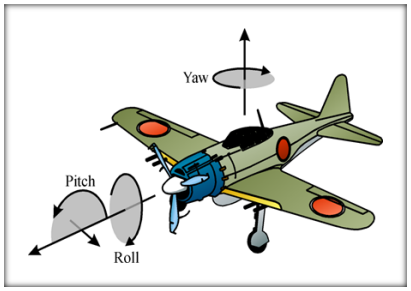
\includegraphics[width=50mm]{src/eulerjevi_koti.png}
    \caption{Eulerjevi koti, vizualno}
    \end{figure}
    Pitch, roll, in yaw so trije osnovni koti rotacije, ki se uporabljajo za opis orientacije telesa v tridimenzionalnem prostoru. V kontekstu Eulerjevih kotov se te rotacije nanašajo na vrtenje okrog treh pravokotnih osi, pogosto imenovanih x, y, in z osi. Eulerjevi koti so kotni parametri, ki definirajo vrtenje objekta z zaporedjem treh rotacij okoli določenih osi. Te rotacije so razdeljene na yaw, pitch, in roll, kar opisuje vrtenje glede na osnovne osi. Pomen osi:
    \begin{itemize}
        \item Yaw: Rotacija okoli navpične osi (Z), sprememba smeri levo-desno.
        \item Pitch: Rotacija okoli prečne osi (Y), dviganje ali spuščanje nosu.
        \item Roll: Rotacija okoli dolžinske osi (X), nagibanje v levo ali desno.
    \end{itemize}
    Eulerjevi koti se definirajo kot sekvenca treh rotacij, običajno v določenem vrstnem redu. Ena pogosta sekvenca je yaw → pitch → roll (rotacije okoli z → y → x osi), kjer vsaka naslednja rotacija vpliva na orientacijo po prejšnji. Vendar obstaja več različnih vrst Eulerjevih kotov, odvisno od izbire vrstnega reda osi.
    \item Kardanska zapora (angl. gimbal lock): izgubimo eno prostorsko stopnjo, če zavrtimo skozi eno os toliko, da bo poravnano z drugo osjo, ker če je 0, bo z vrtenjem tudi ostal pri 0 (zmanjša se število neodvisnih osi, saj dve osi postaneta sočasni). Je pojav, ki se pojavi pri uporabi Eulerjevih kotov za opis rotacij v tridimenzionalnem prostoru. Kardanska zapora nastane, ko se dve rotacijski osi poravnata, kar povzroči izgubo ene stopnje prostosti (degree of freedom) in vodi do nezmožnosti natančnega opisovanja rotacij okoli vseh osi.
    \item Zakonitosti veriženja transformacij:
    \begin{enumerate}
        \item $p' = Mp = M_3M_2M_1p$
        \item $M_3(M_2(M_1p)) = (M_3M_2)M_1p = M_3(M_2M_1)p = (M_3M_2M_1)p$, komutativnost
        \item $p^{'T} = p^TM^T$, transponiranje
        \item $p^{'T} = p^TM_1^TM_2^TM_3^T$, transponiranje, obratni vrstni red
        \begin{figure}[H]
        \centering
        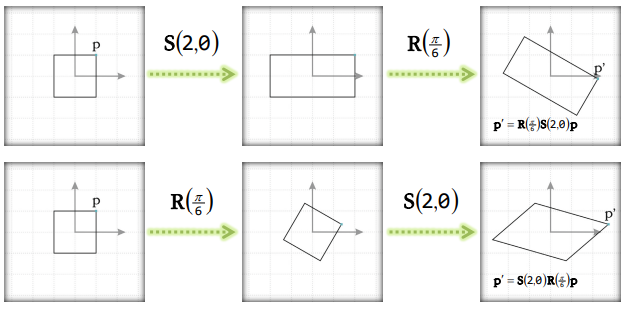
\includegraphics[width=100mm]{src/vrstni_red_verizenja.png}
        \caption{Primer, kako pomemben je vrstni red operacij}
        \end{figure} 
        \item Vrstni red operacij: SRT → skaliranje → vrtenje → premiki (dogovor). Vse operacije izvajamo preko izhodišča
    \end{enumerate}
    \item Transformacije vrtenja okrog poljubne točke: $p' = M_3M_2M_1p$, $p' = T(r)R(\theta)T(-r)p$
        \begin{figure}[H]
        \centering
        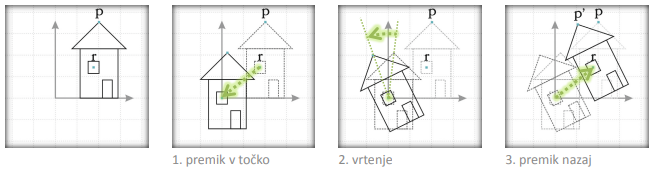
\includegraphics[width=100mm]{src/vrtenje_okrog_poljubne_tocke.png}
        \caption{Postopek vrtenja okoli poljubne točke}
        \end{figure} 
\end{itemize}

\subsection{Toge transformacije}
\begin{itemize}
    \item Vse transformacije, ki spreminjajo lokacijo in orientacijo, vendar ohranjajo obliko objekta (kot, volumen). To sta samo premik in vrtenje.
\end{itemize}

\subsection{Prehodi med koordinatnimi sistemi}
\begin{itemize}
    \item "Točki p, podani v koord. sistemu (x,y,z,o), poišči koordinate glede na koord. sistem (u,v,w,q)"
        \begin{figure}[H]
        \centering
        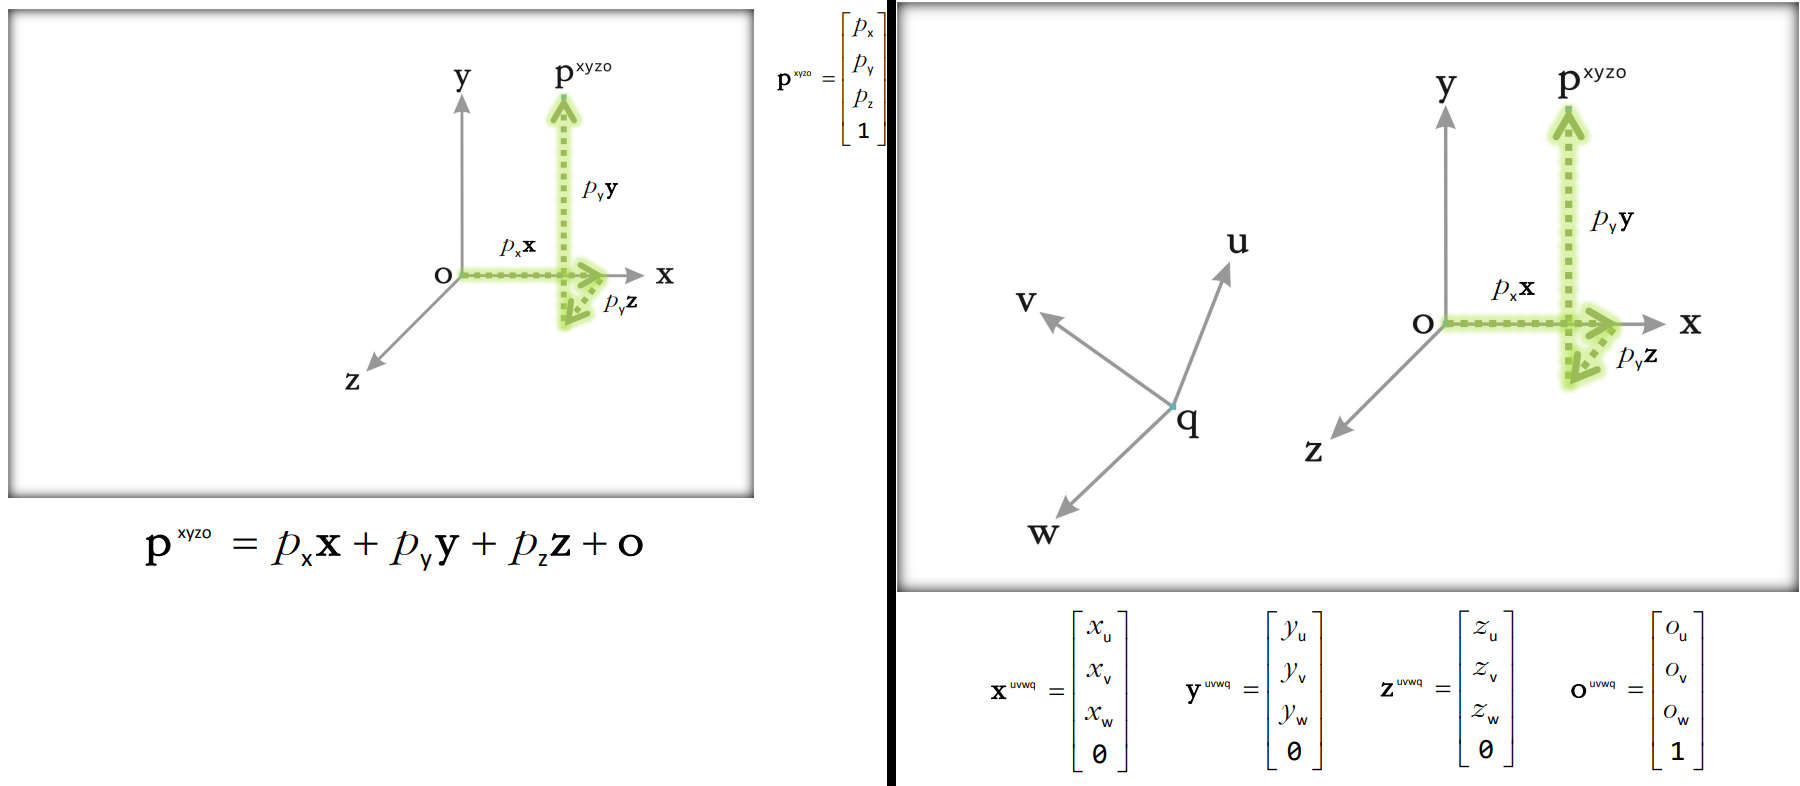
\includegraphics[width=150mm]{src/prehajanje_koord_sistemov_1.png}
        \caption{Predstavitev točke v enem ter v drugem sistemu}
        \end{figure} 
    Tako lahko zapišemo: $p^{uvwq} = p_xx^{uvwq} + p_yy^{uvwq} + p_zz^{uvwq} + o^{uvwq}$, oz. $p^{uvwq} = \begin{bmatrix} x & y & z & o \end{bmatrix} \begin{bmatrix} p_x \\ p_y \\ p_z \\ 1 \end{bmatrix}$ \\
    Kar lahko zapišemo v skupno transformacijsko matriko, hkrati pa dobimo tudi inverz, torej prehod iz (x,y,z,o) v (u,v,w,q) ter nazaj. Pri tem oznaka B pomeni operacije raztega, vrtenja, skaliranja ter striženja. B je tudi ortonorminirana baza, torej je inverz samo transponiranje.
        \begin{figure}[H]
        \centering
        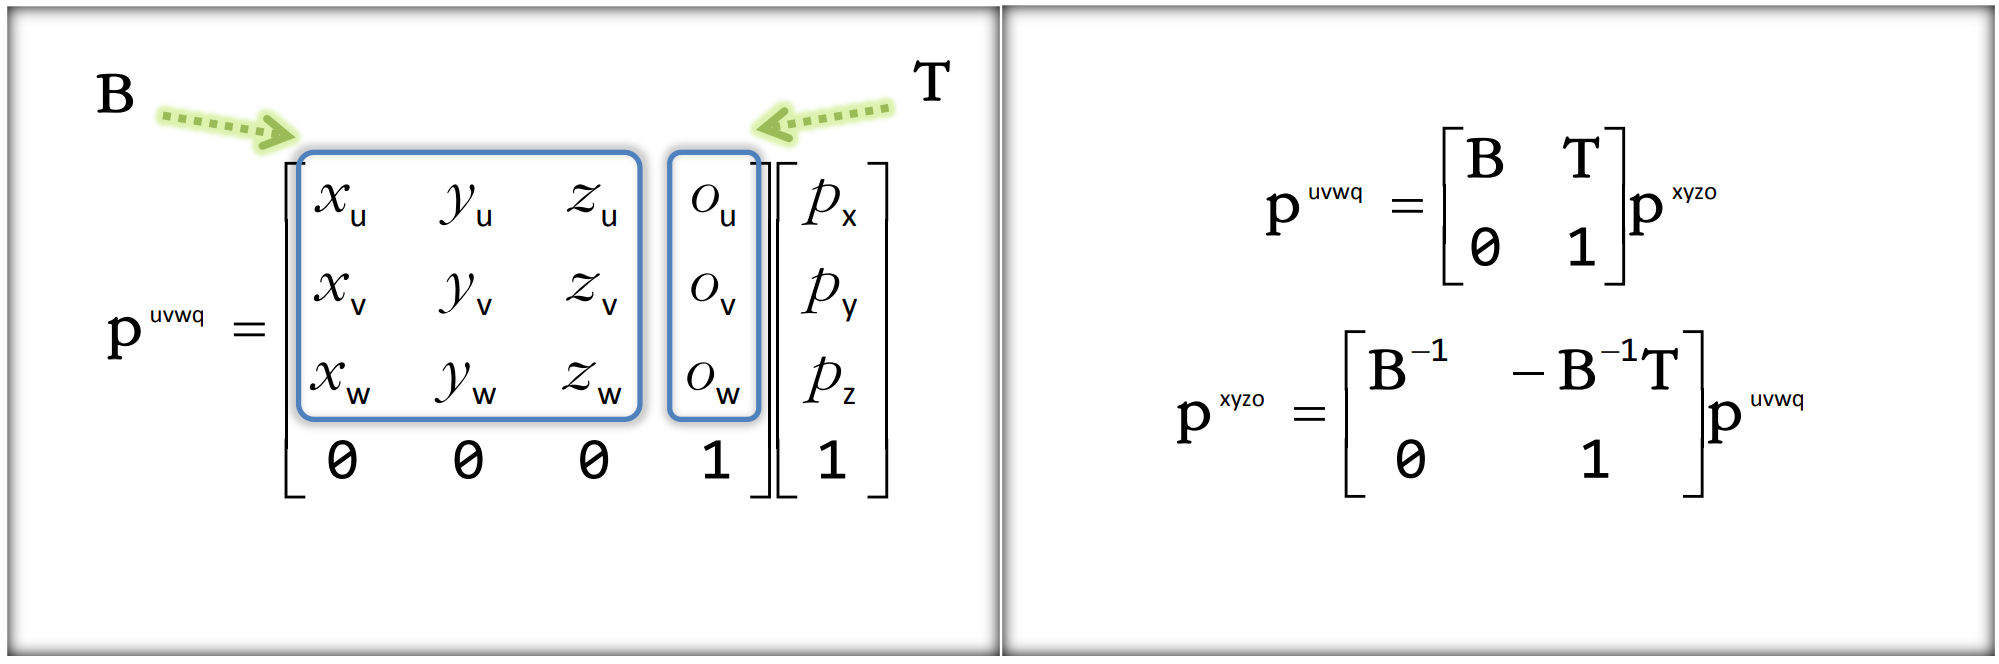
\includegraphics[width=100mm]{src/prehajanje_koord_sistemov_2.png}
        \end{figure} 
\end{itemize}

\section{Projekcije}

\end{document}